\documentclass{report}
\usepackage{blindtext}
\usepackage{multicol}
\usepackage{fancyhdr}
\usepackage{graphicx}
\usepackage{float} % For H placement option
\usepackage{url}  % for citation urls
\usepackage{amsmath} 

\title{Immunosenescence and its Function in Vaccination and Deterministic Mathematical Modeling}
\author{Sahana Balaji \& Brenna Neeland}
\date{May 1, 2024}

\pagestyle{fancy}
\fancyhf{} % Clear header and footer
\rhead{Balaji \& Neeland \thepage}
\lhead{CSCI 4830/7000} % Left header
\begin{document}
\maketitle
\thispagestyle{fancy}
\textbf{Github:} \url{https://github.com/saba2735/Infectious_Disease_Project}

\section*{Introduction}

Varying factors can contribute to susceptibility to disease among populations\. One particular factor to consider is age and the development of immunosenescence. Immunosenescence is the alteration of immune function, typically thymic involution causing the decreased functions of T and B cells, due to aging \cite{rink2022}. Both of these cell types are involved in the acquisition or antigen-specific immune response such that they are the only cells in an organism that can recognize and respond to that specific antigen epitope \cite{cano2013}. In immunosenescence, the number of memory T and B cells increase, while the response to new antigens decreases. Similarly, this decreases the function of granulocytes, macrophages, and NK cells \cite{rink2022}.

The importance of immunosenescence and aging was especially emphasized during the COVID-19 pandemic in 2020. Increased susceptibility to disease due to immunosenescence could play a huge role in the way mathematical and computational methods model disease and immunity as provided by vaccinations. This project seeks to explore how immunosenescence can be mathematically modeled using an SEIRS model, and how this idea can be applied to vaccination models. 

\section*{Methods}
In order to analyze varying susceptibility among different age groups, an SEIRS model was formed and modified to include variable T. T represents varying loss of immunity due to immunosenescence. This allowed us to form a set of ordinary differential equations (ODEs) with a varied T based on age.

Furthermore, a contact matrix was formed to better understand the contacts that occur between the three different age groups.(figure 3). 

We then generated a leaky vaccine model using varying R0 values for influenza. Influenza was chosen as there was a lot of data provided for different age groups in terms of $R_0$ values. $R_0$ values for kids varied between 1.7-2, for adults varied between 1-2 and for grandparents varied between 1-1.4. Additionally, the code took into account 145 people. Of these 145 people there were 30 kids, 55 parents, and 60 grandparents. The different ranges of R0 values and the varying number of people in each group were manipulated together to analyze the leaky model of a vaccine when Vaccine Efficacy (Ve) was varying. The different VE values that were looked into were 0,0.8 and 1. It was then determined what the total infection would be based on the varying VE values and $R_0$ values provided for each group. We then saved these results to a CSV file (\texttt{simulation\_results.csv}).Each age group was visualized using bar charts generated with the Matplotlib library in Python.

 The \(R_{0}\) values and the total infections from the leaky vaccine model were visualized among varying age groups using bar charts via seaborn library in Python. 

 After analyzing the leaky vaccine model, we then analyzed the rate of secondary infections or \(R_{E}\). This value determines the average number of secondary infections generated by a single infectious individual in a population where some individuals may be immune or have reduced susceptibility due to factors such as vaccination or prior infection. The \(R_{E}\) values was calculated in python. All assumptions made in the leaky vaccine model such as number of people in the population, the \(R_{0}\) values and the VE values stayed the same. These values were then exported to a CSV file. This made it easier to view the difference between the \(R_{0}\) value and the \(R_{E}\)value. 

\section*{Results}
We first analyzed the SEIRS model to understand how the current model is failing to model immunosenescence (figure 1). A variable to model loss of immunity needs to be considered to understand variations in loss of immunity due to immunosenescence and aging overall.

\begin{figure}[H]
    \centering
    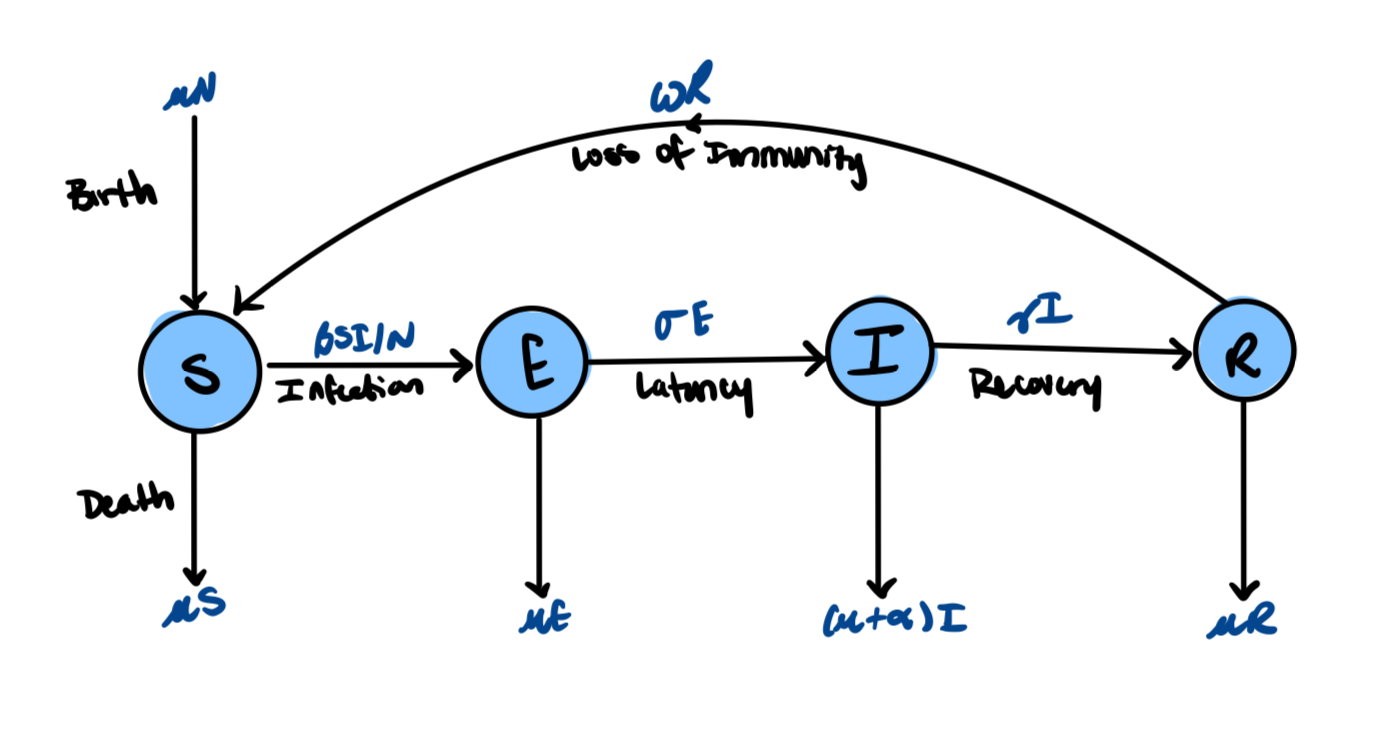
\includegraphics[width=0.8\textwidth]{seirs.jpeg}
    \caption{SEIRS Model}
    \label{fig:SEIRS}
\end{figure}

\begin{align}
\frac{dS}{dt} &= \mu N - \beta S \frac{I}{N} + \omega R - \mu S \\
\frac{dE}{dt} &= \beta S \frac{I}{N} - \sigma E - \mu E \\
\frac{dI}{dt} &= \sigma E - \gamma I - ( \mu + \alpha )I \\
\frac{dR}{dt} &= \gamma I - \omega R - \mu R
\end{align}

where:
\begin{itemize}
  \item \(S\) represents the number of susceptible individuals,
  \item \(E\) represents the number of exposed (but not yet infectious) individuals,
  \item \(I\) represents the number of infectious individuals,
  \item \(R\) represents the number of removed (either recovered or deceased) individuals,
  \item \(N\) represents the total population size.
\end{itemize}


 This led us to form a SEIRS model to include variable 'T' which includes some form of timestep in order to anaylze loss of immunity. This allowed us to adjust the model equations such that if an individual has an increased loss of immunity due to age it can be included within this variable (figure 2).
 
% JPEGs
\begin{figure}[H]
    \centering
    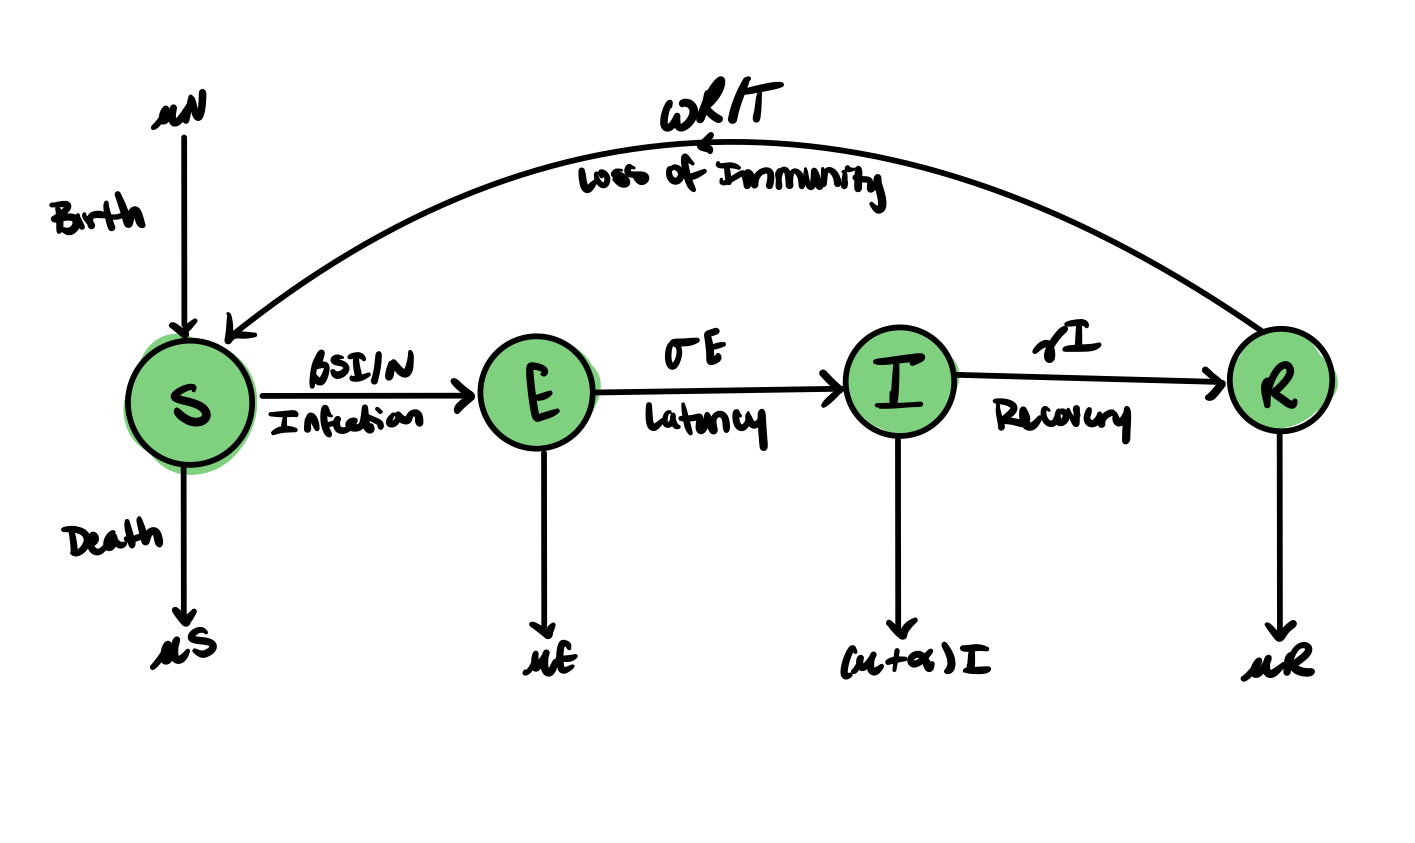
\includegraphics[width=0.8\textwidth]{seirsM.jpeg}
    \caption{Modified SEIRS Model}
    \label{fig:Immunosenscence Model}
\end{figure}
\begin{align}
\frac{dS}{dt} &= \mu N - \beta S \frac{I}{N} + \omega \frac{R}{T} - \mu S \\
\frac{dE}{dt} &= \beta S \frac{I}{N} - \sigma E - \mu E \\
\frac{dI}{dt} &= \sigma E - \gamma I - ( \mu + \alpha )I \\
\frac{dR}{dt} &= \gamma I - \omega \frac{R}{T} - \mu R
\end{align}

where:
\begin{itemize}
  \item \(S\) represents the number of susceptible individuals,
  \item \(E\) represents the number of exposed (but not yet infectious) individuals,
  \item \(I\) represents the number of infectious individuals,
  \item \(R\) represents the number of removed (either recovered or deceased) individuals,
  \item \(N\) represents the total population size,
  \item \(T\) represents the time in which immunity lasts
\end{itemize}

The formation of these equations allows us to consider a time period in which immunity remains. For example immunity for the elderly may be decreased, and now our equations can compensate for this change. 

In figure 3 the contact matrix that was created made a few assumptions. It was suggested that kids come into contact with 20 kids a day, 2 parents a day and 2 grandparents a day. Parents come into contact with 2 kids a day, 1 parent a day, and 2 grandparents a day. Grandparents come into contact with 2 kids a day, 2 parents a day and 1 grandparent a day. 

\begin{figure}[H]
    \centering
    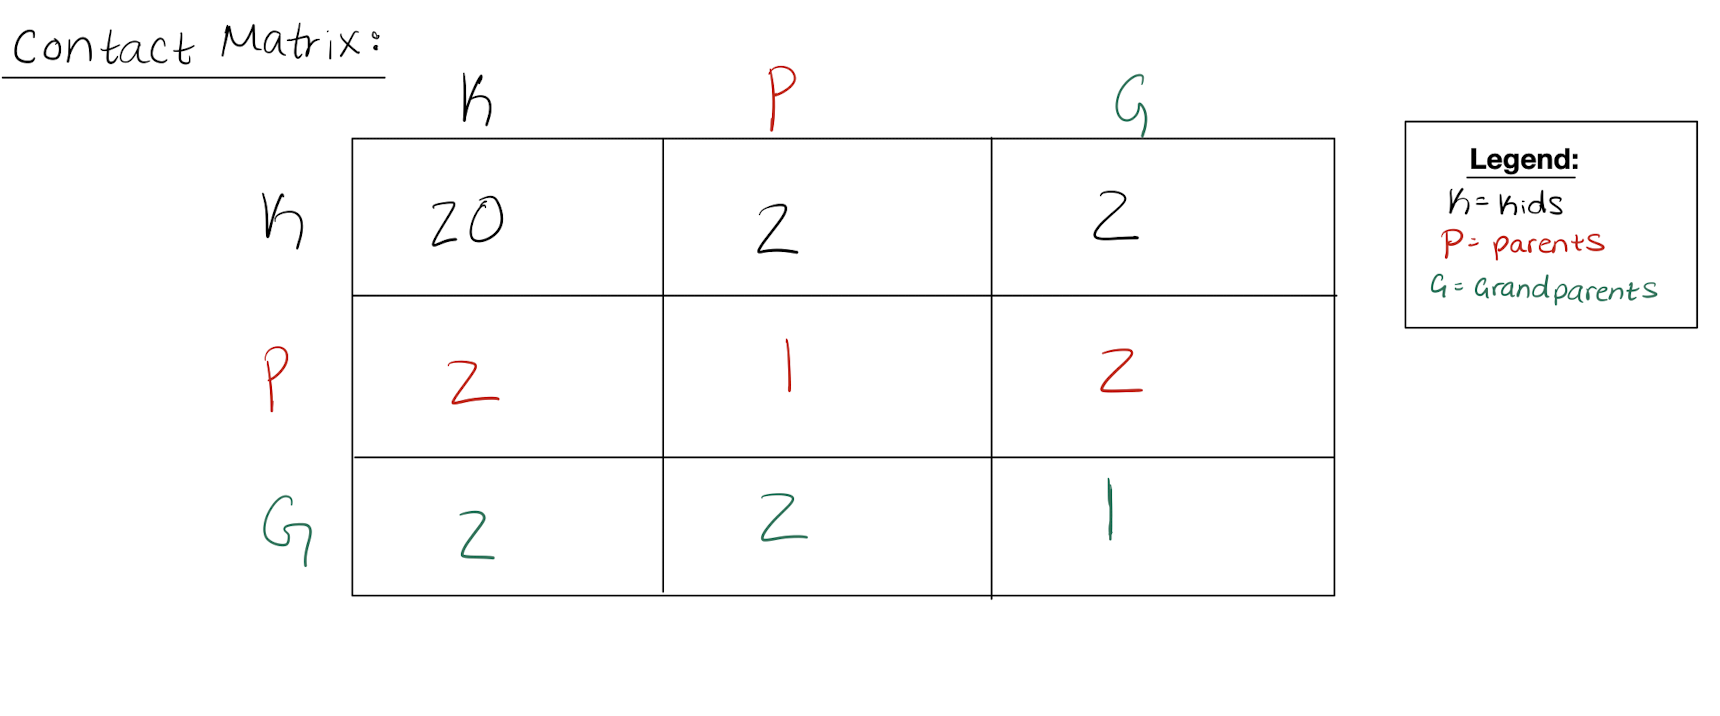
\includegraphics[width=0.8\textwidth]{Contact_Matrix.png}
    \caption{Contact Matrix for Each Age Group}
    \label{fig:Contact Matrix}
\end{figure}
In figures 4-6 bar charts for varying Vaccine Efficacy (VE) can be observed for various \(R_{0}\) values. Each result is separated by age group. Our analysis shows supports that with increased VE less individuals are likely to get infected. Furthermore, kids tended to have increased total infections at a VE of 0.8 compared to both adults and grandparents (figure 4). Grandparents and adults had similar infections totals (figure 5 and 6).

%PNGs
\begin{figure}[H]
    \centering
    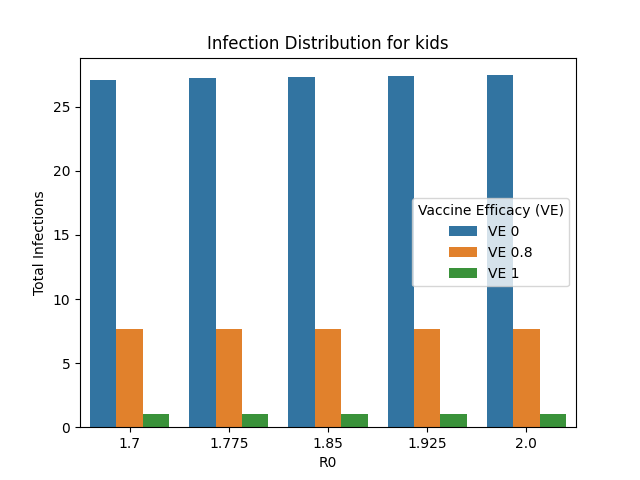
\includegraphics[width=0.8\textwidth]{kids.png}
    \caption{{Varying Vaccine Efficacy for Kids for Ranging \(R_{0}\) Values}}
    \label{fig:kids} 
\end{figure}
\begin{figure}[H]
    \centering
    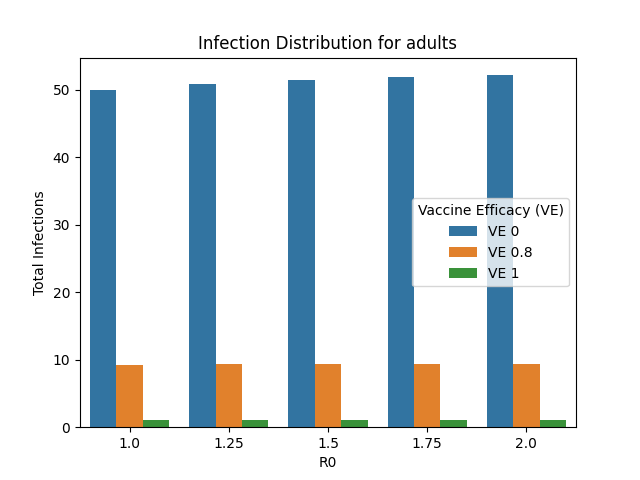
\includegraphics[width=0.8\textwidth]{adults.png}
    \caption{Varying Vaccine Efficacy for Adults for Ranging \(R_{0}\) Values} % Enclose R_{0} in math mode
    \label{fig:adults} % Add label for referencing
\end{figure}
\begin{figure}[H]
    \centering
    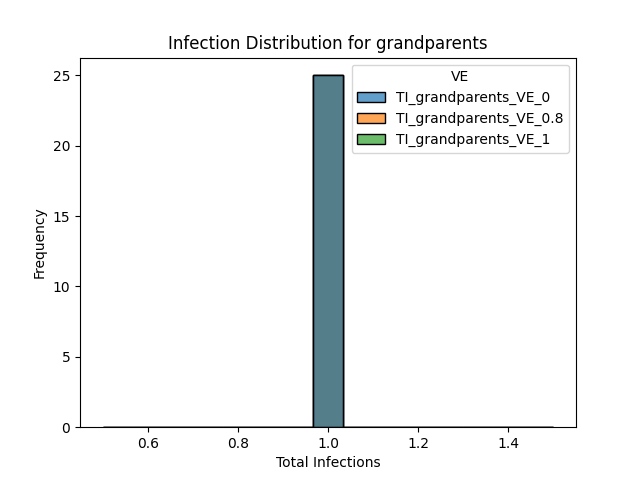
\includegraphics[width=0.8\textwidth]{grandparents.png}
    \caption{{Varying Vaccine Efficacy for Grandparents for Ranging \(R_{0}\) Values}}
    \label{fig:grandparents} 
\end{figure}
Figures 7-9 show bar charts that are comparing \(R_{0}\) and \(R_{E}\) for our age groups. We can observe that kids were the most susceptible group closely followed by grandparents and then adults. 
\begin{figure}[H]
    \centering
    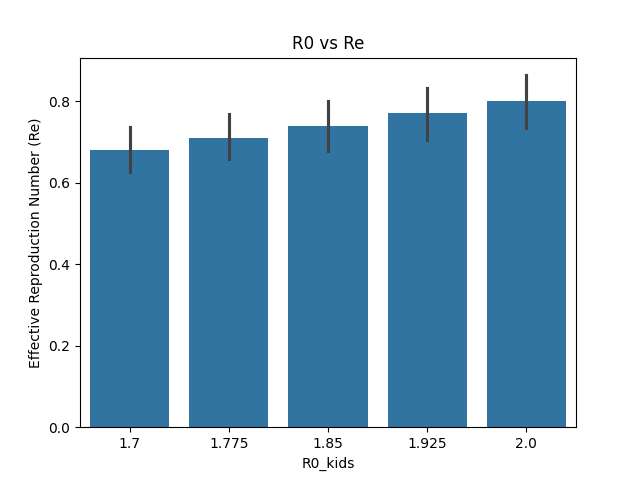
\includegraphics[width=0.8\textwidth]{re_kids.png}
    \caption{Comparison of \(R_{0}\) and \(R_{E}\) for Kids}
    \label{fig:barkids} 
\end{figure}
\begin{figure}[H]
    \centering
    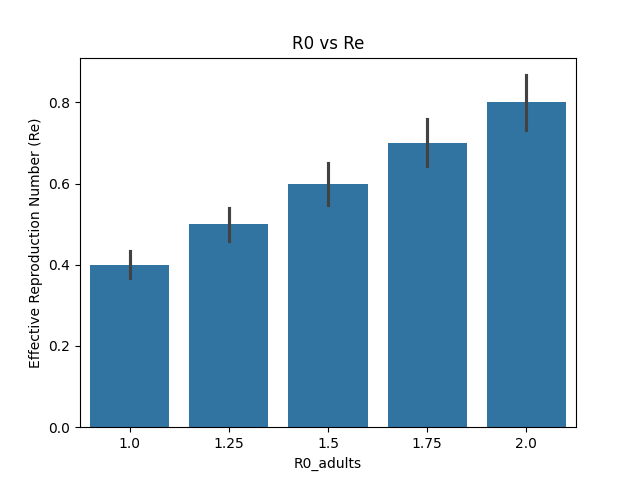
\includegraphics[width=0.8\textwidth]{re_adults.png}
    \caption{Comparison of \(R_{0}\) and \(R_{E}\) for Adults}
    \label{fig:baradults} 
\end{figure}
\begin{figure}[H]
    \centering
    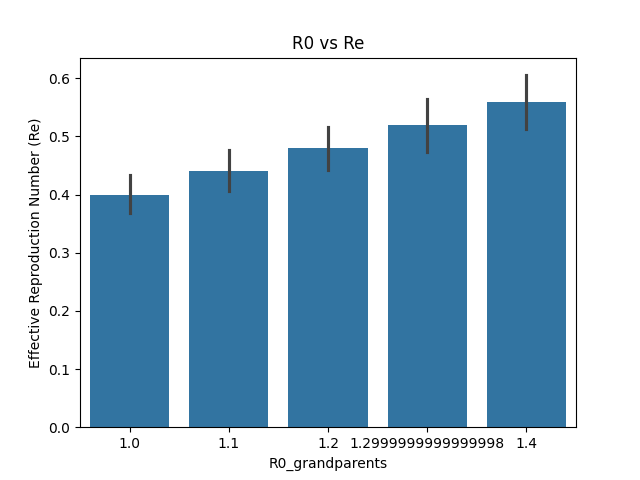
\includegraphics[width=0.8\textwidth]{re_grandparents.png}
    \caption{Comparison of \(R_{0}\) and \(R_{E}\) for Grandparents}
    \label{fig:bargrandparents} 
\end{figure}

\section*{Conclusion}
Modeling immunosensescence can help us form mathematical models for molecular cascading processes and signal transduction and its role in susceptibility to pathogens. The function of T and B cells in immune response is crucial and their decreased function in aging populations is incredibly important to vaccination models and strategies.

Based on the data, when Vaccine Efficacy (VE) is 0 most of the population becomes infected. This is consistence since the vaccine is not effective or the same as if no one is vaccinated. Therefore, most of the population will become infected. However, when VE was simulated as 0.8 only about 20\% of the population became infected. When everyone is vaccinated and the VE is about 80\% about 20\% of the population should become infected despite being vaccinated. When we model VE as 1, everyone is vaccinated with 100\% vaccine efficacy. Therefore, no one should be infected even when exposed to one individual who is. In our simulation only one individual who be infected due to this assumption.

Furthermore, when considering $R_E$ it can be suggested that kids and grandparents were more susceptible to primary and secondary infections than adults. We can then hypothesize that kids will have lowered immunity due to age and being constantly exposed to new bacteria. Similarly, adults who are healthy should be less susceptible due to proper T and B cell function and proper antigen-response when exposed to pathogens. Furthermore, the elderly should be more susceptible than adults due to immunosenescence which causes decreased T and B cell function. Our data is consistent with this hypothesis as adults were observed to be the least susceptible to both primary and secondary infections, followed by grandparents, with kids being the most susceptible.

\section*{Discussion}
One main challenge is individuality. Everyone is different and respond differently to exposure to pathogens resulting in varying outcomes. In the future a Leaky Vaccination Model should be produced for the SEIRS model to truly understand the loss of immunity for both vaccinations and the role that immunosenescence plays in this. It is important to consider the incubation period as it can be different for the various age groups. For kids and grandparents the incubation period may be shorter than the incubation period in adults. In the vaccine model it is also important to discuss the waning period of a vaccine as that will also vary amongst the different age groups. The waning period of vaccine can help determine the possibility of when an individual from a given age group is no longer prevented from the disease and when they can be in the susceptible group again. 

A larger data set should be considered as well. This can help us to understand population dynamics, the number of people in each group needs to increase.
Furthermore, making a snakemake file or a pipeline to simulate the data and make it easier to handle the population in the different age groups. Finally, making a good outline for an SEIRS model so that the model can be changed based on the disease. In the future if an epidemic were to occur, this model can be a good framework of how to implement modeling immunosenescence, so that vaccination recommendation can be made easier. 

Some limitations of this study is the assumptions that deterministic models make. As mentioned prior, no individual is the same. Likewise, susceptibility changes from individual to individual due to various factors. For example, chronic disease, increased contact with infectious individuals, and access to medicine and medical care. These limitations are important to understand when using these models since not one fits all.


\begin{thebibliography}{}

\bibitem{bjornstad2020} 
Bjørnstad, O.N., Shea, K., Krzywinski, M., et al. (2020). The SEIRS model for infectious disease dynamics. \textit{Nat Methods, 17}, 557–558. \url{https://doi.org/10.1038/s41592-020-0856-2}

\bibitem{cano2013} 
Cano, R. L. E., \& Lopera, H. D. E. (2013). Introduction to T and B lymphocytes. In \textit{Autoimmunity: From Bench to Bedside} [Internet]. Retrieved from \url{https://www.ncbi.nlm.nih.gov/books/NBK459471/}

\bibitem{frontiers2022} 
Frontiers in Immunology. (2022). Tissue-Resident Macrophages in the Control of Infection and Tissue Repair. \textit{Frontiers in Immunology, 13}, 942796. \url{https://doi.org/10.3389/fimmu.2022.942796}

\bibitem{whitfield2020} 
Whitfield, J.M., Onken, M.D., Larsen, M.V., et al. (2020). CRISPR meets single-cell genomics: a multi-dimensional perspective. \textit{Seminars in Immunopathology, 42}(2), 177-188. \url{https://doi.org/10.1007/s00281-020-00824-x}

\bibitem{liu2023} 
Liu, Z., Liang, Q., Ren, Y., et al. (2023). Immunosenescence: molecular mechanisms and diseases. \textit{Sig Transduct Target Ther, 8}, 200. \url{https://doi.org/10.1038/s41392-023-01451-2}

\bibitem{mittelbrunn2021} 
Mittelbrunn, M., Kroemer, G. (2021). Hallmarks of T cell aging. \textit{Nat Immunol, 22}, 687–698. \url{https://doi.org/10.1038/s41590-021-00927-z}

\bibitem{epidemiology2019} 
Principles of Epidemiology. (2019, December 2). National Center for Biotechnology Information. \url{https://www.ncbi.nlm.nih.gov/books/NBK459471/}

\bibitem{rink2022} 
Rink, L., \& Wessels, I. (2022). Immunosenescence. In N. Rezaei (Ed.), Encyclopedia of Infection and Immunity (pp. 259-276). Elsevier. \url{https://doi.org/10.1016/B978-0-12-818731-9.00072-0}

\bibitem{treaty} 
Towards an international treaty on pandemics. (n.d.). European Council - Council of the European Union. \url{consilium.europa.eu/en/infographics/towards-an-international-treaty-on-pandemics/}

\bibitem{yousefzadeh2021} 
Yousefzadeh, M.J., Flores, R.R., Zhu, Y., et al. (2021). An aged immune system drives senescence and ageing of solid organs. \textit{Nature, 594}, 100–105. \url{https://doi.org/10.1038/s41586-021-03547-7}

\end{thebibliography}
\end{document}
